\documentclass[twoside]{book}

% Packages required by doxygen
\usepackage{calc}
\usepackage{doxygen}
\usepackage{graphicx}
\usepackage[utf8]{inputenc}
\usepackage{makeidx}
\usepackage{multicol}
\usepackage{multirow}
\usepackage{textcomp}
\usepackage[table]{xcolor}

% Font selection
\usepackage[T1]{fontenc}
\usepackage{mathptmx}
\usepackage[scaled=.90]{helvet}
\usepackage{courier}
\usepackage{amssymb}
\usepackage{sectsty}
\renewcommand{\familydefault}{\sfdefault}
\allsectionsfont{%
  \fontseries{bc}\selectfont%
  \color{darkgray}%
}
\renewcommand{\DoxyLabelFont}{%
  \fontseries{bc}\selectfont%
  \color{darkgray}%
}

% Page & text layout
\usepackage{geometry}
\geometry{%
  a4paper,%
  top=2.5cm,%
  bottom=2.5cm,%
  left=2.5cm,%
  right=2.5cm%
}
\tolerance=750
\hfuzz=15pt
\hbadness=750
\setlength{\emergencystretch}{15pt}
\setlength{\parindent}{0cm}
\setlength{\parskip}{0.2cm}
\makeatletter
\renewcommand{\paragraph}{%
  \@startsection{paragraph}{4}{0ex}{-1.0ex}{1.0ex}{%
    \normalfont\normalsize\bfseries\SS@parafont%
  }%
}
\renewcommand{\subparagraph}{%
  \@startsection{subparagraph}{5}{0ex}{-1.0ex}{1.0ex}{%
    \normalfont\normalsize\bfseries\SS@subparafont%
  }%
}
\makeatother

% Headers & footers
\usepackage{fancyhdr}
\pagestyle{fancyplain}
\fancyhead[LE]{\fancyplain{}{\bfseries\thepage}}
\fancyhead[CE]{\fancyplain{}{}}
\fancyhead[RE]{\fancyplain{}{\bfseries\leftmark}}
\fancyhead[LO]{\fancyplain{}{\bfseries\rightmark}}
\fancyhead[CO]{\fancyplain{}{}}
\fancyhead[RO]{\fancyplain{}{\bfseries\thepage}}
\fancyfoot[LE]{\fancyplain{}{}}
\fancyfoot[CE]{\fancyplain{}{}}
\fancyfoot[RE]{\fancyplain{}{\bfseries\scriptsize Generated on Sun Dec 7 2014 00\-:21\-:52 for Battle-\/\-Ship by Doxygen }}
\fancyfoot[LO]{\fancyplain{}{\bfseries\scriptsize Generated on Sun Dec 7 2014 00\-:21\-:52 for Battle-\/\-Ship by Doxygen }}
\fancyfoot[CO]{\fancyplain{}{}}
\fancyfoot[RO]{\fancyplain{}{}}
\renewcommand{\footrulewidth}{0.4pt}
\renewcommand{\chaptermark}[1]{%
  \markboth{#1}{}%
}
\renewcommand{\sectionmark}[1]{%
  \markright{\thesection\ #1}%
}

% Indices & bibliography
\usepackage{natbib}
\usepackage[titles]{tocloft}
\setcounter{tocdepth}{3}
\setcounter{secnumdepth}{5}
\makeindex

% Hyperlinks (required, but should be loaded last)
\usepackage{ifpdf}
\ifpdf
  \usepackage[pdftex,pagebackref=true]{hyperref}
\else
  \usepackage[ps2pdf,pagebackref=true]{hyperref}
\fi
\hypersetup{%
  colorlinks=true,%
  linkcolor=blue,%
  citecolor=blue,%
  unicode%
}

% Custom commands
\newcommand{\clearemptydoublepage}{%
  \newpage{\pagestyle{empty}\cleardoublepage}%
}


%===== C O N T E N T S =====

\begin{document}

% Titlepage & ToC
\hypersetup{pageanchor=false}
\pagenumbering{roman}
\begin{titlepage}
\vspace*{7cm}
\begin{center}%
{\Large Battle-\/\-Ship }\\
\vspace*{1cm}
{\large Generated by Doxygen 1.8.6}\\
\vspace*{0.5cm}
{\small Sun Dec 7 2014 00:21:52}\\
\end{center}
\end{titlepage}
\clearemptydoublepage
\tableofcontents
\clearemptydoublepage
\pagenumbering{arabic}
\hypersetup{pageanchor=true}

%--- Begin generated contents ---
\chapter{Hierarchical Index}
\section{Class Hierarchy}
This inheritance list is sorted roughly, but not completely, alphabetically\-:\begin{DoxyCompactList}
\item \contentsline{section}{battle\-Ship.\-Battle\-Ship}{\pageref{classbattleShip_1_1BattleShip}}{}
\item \contentsline{section}{battle\-Ship.\-Board}{\pageref{classbattleShip_1_1Board}}{}
\item \contentsline{section}{battle\-Ship.\-Player}{\pageref{classbattleShip_1_1Player}}{}
\begin{DoxyCompactList}
\item \contentsline{section}{battle\-Ship.\-Computer\-Player}{\pageref{classbattleShip_1_1ComputerPlayer}}{}
\item \contentsline{section}{battle\-Ship.\-Human\-Player}{\pageref{classbattleShip_1_1HumanPlayer}}{}
\end{DoxyCompactList}
\item Window\-Listener\begin{DoxyCompactList}
\item \contentsline{section}{battle\-Ship.\-Window}{\pageref{classbattleShip_1_1Window}}{}
\end{DoxyCompactList}
\end{DoxyCompactList}

\chapter{Class Index}
\section{Class List}
Here are the classes, structs, unions and interfaces with brief descriptions\-:\begin{DoxyCompactList}
\item\contentsline{section}{\hyperlink{classbattleShip_1_1BattleShip}{battle\-Ship.\-Battle\-Ship} \\*This \hyperlink{classbattleShip_1_1BattleShip}{Battle\-Ship} class will implement the game \hyperlink{classbattleShip_1_1BattleShip}{Battle\-Ship} }{\pageref{classbattleShip_1_1BattleShip}}{}
\item\contentsline{section}{\hyperlink{classbattleShip_1_1Board}{battle\-Ship.\-Board} \\*This class is a template for a \hyperlink{classbattleShip_1_1Board}{Board} object }{\pageref{classbattleShip_1_1Board}}{}
\item\contentsline{section}{\hyperlink{classbattleShip_1_1ComputerPlayer}{battle\-Ship.\-Computer\-Player} \\*This will implement an artificial player that can play Battleship }{\pageref{classbattleShip_1_1ComputerPlayer}}{}
\item\contentsline{section}{\hyperlink{classbattleShip_1_1HumanPlayer}{battle\-Ship.\-Human\-Player} \\*This class represents a \hyperlink{classbattleShip_1_1HumanPlayer}{Human\-Player} that can play from a \hyperlink{classbattleShip_1_1Window}{Window} }{\pageref{classbattleShip_1_1HumanPlayer}}{}
\item\contentsline{section}{\hyperlink{classbattleShip_1_1Player}{battle\-Ship.\-Player} \\*This base \hyperlink{classbattleShip_1_1Player}{Player} class is used as a template for it's children }{\pageref{classbattleShip_1_1Player}}{}
\item\contentsline{section}{\hyperlink{classbattleShip_1_1Window}{battle\-Ship.\-Window} }{\pageref{classbattleShip_1_1Window}}{}
\end{DoxyCompactList}

\chapter{Class Documentation}
\hypertarget{classbattleShip_1_1BattleShip}{\section{battle\-Ship.\-Battle\-Ship Class Reference}
\label{classbattleShip_1_1BattleShip}\index{battle\-Ship.\-Battle\-Ship@{battle\-Ship.\-Battle\-Ship}}
}


This \hyperlink{classbattleShip_1_1BattleShip}{Battle\-Ship} class will implement the game \hyperlink{classbattleShip_1_1BattleShip}{Battle\-Ship}.  


\subsection*{Public Member Functions}
\begin{DoxyCompactItemize}
\item 
\hyperlink{classbattleShip_1_1BattleShip_a1f66570b4684f41b7e2e75cc0ee1a50a}{Battle\-Ship} (int rows, int columns)
\begin{DoxyCompactList}\small\item\em Construct a new \hyperlink{classbattleShip_1_1BattleShip}{Battle\-Ship} object. \end{DoxyCompactList}\item 
void \hyperlink{classbattleShip_1_1BattleShip_a9601c44353f90a26d8112bf4cbe93241}{setup\-Players} ()
\begin{DoxyCompactList}\small\item\em Get the players ready to play the game the completion of this method requires that all players are ready to play. \end{DoxyCompactList}\item 
\hypertarget{classbattleShip_1_1BattleShip_a011f43e5b4f5e3897bf77b2926e0d54b}{void \hyperlink{classbattleShip_1_1BattleShip_a011f43e5b4f5e3897bf77b2926e0d54b}{play} ()}\label{classbattleShip_1_1BattleShip_a011f43e5b4f5e3897bf77b2926e0d54b}

\begin{DoxyCompactList}\small\item\em Lets play the game! \end{DoxyCompactList}\end{DoxyCompactItemize}
\subsection*{Static Public Member Functions}
\begin{DoxyCompactItemize}
\item 
static void \hyperlink{classbattleShip_1_1BattleShip_aa9bf43c6d5d03b765441389c3cf091c3}{main} (String\mbox{[}$\,$\mbox{]} args)
\begin{DoxyCompactList}\small\item\em This is the entry point of our program! \end{DoxyCompactList}\end{DoxyCompactItemize}


\subsection{Detailed Description}
This \hyperlink{classbattleShip_1_1BattleShip}{Battle\-Ship} class will implement the game \hyperlink{classbattleShip_1_1BattleShip}{Battle\-Ship}. 

\begin{DoxyAuthor}{Author}
john 
\end{DoxyAuthor}


\subsection{Constructor \& Destructor Documentation}
\hypertarget{classbattleShip_1_1BattleShip_a1f66570b4684f41b7e2e75cc0ee1a50a}{\index{battle\-Ship\-::\-Battle\-Ship@{battle\-Ship\-::\-Battle\-Ship}!Battle\-Ship@{Battle\-Ship}}
\index{Battle\-Ship@{Battle\-Ship}!battleShip::BattleShip@{battle\-Ship\-::\-Battle\-Ship}}
\subsubsection[{Battle\-Ship}]{\setlength{\rightskip}{0pt plus 5cm}battle\-Ship.\-Battle\-Ship.\-Battle\-Ship (
\begin{DoxyParamCaption}
\item[{int}]{rows, }
\item[{int}]{columns}
\end{DoxyParamCaption}
)}}\label{classbattleShip_1_1BattleShip_a1f66570b4684f41b7e2e75cc0ee1a50a}


Construct a new \hyperlink{classbattleShip_1_1BattleShip}{Battle\-Ship} object. 


\begin{DoxyParams}{Parameters}
{\em rows} & How many rows are in the board? \\
\hline
{\em columns} & How many columns are in the board? \\
\hline
\end{DoxyParams}


\subsection{Member Function Documentation}
\hypertarget{classbattleShip_1_1BattleShip_aa9bf43c6d5d03b765441389c3cf091c3}{\index{battle\-Ship\-::\-Battle\-Ship@{battle\-Ship\-::\-Battle\-Ship}!main@{main}}
\index{main@{main}!battleShip::BattleShip@{battle\-Ship\-::\-Battle\-Ship}}
\subsubsection[{main}]{\setlength{\rightskip}{0pt plus 5cm}static void battle\-Ship.\-Battle\-Ship.\-main (
\begin{DoxyParamCaption}
\item[{String\mbox{[}$\,$\mbox{]}}]{args}
\end{DoxyParamCaption}
)\hspace{0.3cm}{\ttfamily [static]}}}\label{classbattleShip_1_1BattleShip_aa9bf43c6d5d03b765441389c3cf091c3}


This is the entry point of our program! 


\begin{DoxyParams}{Parameters}
{\em args} & Program arguments \\
\hline
\end{DoxyParams}
\hypertarget{classbattleShip_1_1BattleShip_a9601c44353f90a26d8112bf4cbe93241}{\index{battle\-Ship\-::\-Battle\-Ship@{battle\-Ship\-::\-Battle\-Ship}!setup\-Players@{setup\-Players}}
\index{setup\-Players@{setup\-Players}!battleShip::BattleShip@{battle\-Ship\-::\-Battle\-Ship}}
\subsubsection[{setup\-Players}]{\setlength{\rightskip}{0pt plus 5cm}void battle\-Ship.\-Battle\-Ship.\-setup\-Players (
\begin{DoxyParamCaption}
{}
\end{DoxyParamCaption}
)}}\label{classbattleShip_1_1BattleShip_a9601c44353f90a26d8112bf4cbe93241}


Get the players ready to play the game the completion of this method requires that all players are ready to play. 

Make sure both players are ready, if they aren't then we should wait 1 second.

The documentation for this class was generated from the following file\-:\begin{DoxyCompactItemize}
\item 
/home/john/\-Workspaces/\-Java/\-Battle-\/\-Ship/src/battle\-Ship/Battle\-Ship.\-java\end{DoxyCompactItemize}

\hypertarget{classbattleShip_1_1Board}{\section{battle\-Ship.\-Board Class Reference}
\label{classbattleShip_1_1Board}\index{battle\-Ship.\-Board@{battle\-Ship.\-Board}}
}


This class is a template for a \hyperlink{classbattleShip_1_1Board}{Board} object.  


\subsection*{Public Member Functions}
\begin{DoxyCompactItemize}
\item 
\hyperlink{classbattleShip_1_1Board_ab29903dca128c549a04ef1bd8a03e284}{Board} (int rows, int columns)
\begin{DoxyCompactList}\small\item\em Create a new \hyperlink{classbattleShip_1_1Board}{Board} object with the specified amount of rows and columns. \end{DoxyCompactList}\item 
void \hyperlink{classbattleShip_1_1Board_a37632e4b600f3bcb1b196c90d7371a62}{print} (\hyperlink{classbattleShip_1_1Window}{Window} window)
\begin{DoxyCompactList}\small\item\em Print the board out to a window. \end{DoxyCompactList}\item 
int \hyperlink{classbattleShip_1_1Board_a7f3ee785960f0a29eb066a0cc76e925b}{place\-Piece} (int start\-Row, int start\-Col, int ship\-Code, boolean vertical)
\begin{DoxyCompactList}\small\item\em Places the piece on the board. \end{DoxyCompactList}\item 
\hypertarget{classbattleShip_1_1Board_aa6205fe92d7e29d281c383f5e57384ad}{int {\bfseries get\-Columns} ()}\label{classbattleShip_1_1Board_aa6205fe92d7e29d281c383f5e57384ad}

\item 
\hypertarget{classbattleShip_1_1Board_aec4594650e89c01f94f43851d81ea887}{int {\bfseries get\-Rows} ()}\label{classbattleShip_1_1Board_aec4594650e89c01f94f43851d81ea887}

\end{DoxyCompactItemize}
\subsection*{Static Public Attributes}
\begin{DoxyCompactItemize}
\item 
static final char \hyperlink{classbattleShip_1_1Board_a1182aaa1c9965e82514001411e92deda}{bup} = '$^\wedge$'
\begin{DoxyCompactList}\small\item\em Up symbol for a ship. \end{DoxyCompactList}\item 
static final char \hyperlink{classbattleShip_1_1Board_a0fdd0fa1e2c590cccc27daf05aa9cf6b}{bdown} = 'v'
\begin{DoxyCompactList}\small\item\em Down symbol for a ship. \end{DoxyCompactList}\item 
static final char \hyperlink{classbattleShip_1_1Board_a9d97dd87cddd014a15af04801920d50e}{bright} = '$>$'
\begin{DoxyCompactList}\small\item\em Right symbol for a ship. \end{DoxyCompactList}\item 
static final char \hyperlink{classbattleShip_1_1Board_a6db9e34520009f40729eb730ee6cb509}{bleft} = '$<$'
\begin{DoxyCompactList}\small\item\em Left symbol for a ship. \end{DoxyCompactList}\item 
static final char \hyperlink{classbattleShip_1_1Board_a73ed34c95d608cdb748ff950841307d7}{bhull} = '$\ast$'
\begin{DoxyCompactList}\small\item\em Hull symbol for a ship. \end{DoxyCompactList}\item 
static final char \hyperlink{classbattleShip_1_1Board_a46a888460556cbefb33d9cb048a610fc}{hit} = 'X'
\begin{DoxyCompactList}\small\item\em Hit symbol. \end{DoxyCompactList}\item 
static final char \hyperlink{classbattleShip_1_1Board_a8c0a9cd8bd0c3829c01dccd8466c8ee6}{miss} = 'o'
\begin{DoxyCompactList}\small\item\em Miss symbol. \end{DoxyCompactList}\item 
static final char \hyperlink{classbattleShip_1_1Board_ae9d384309243340b7daf402ab99175df}{bnone} = ' '
\begin{DoxyCompactList}\small\item\em Empty spot symbol. \end{DoxyCompactList}\item 
static final int\mbox{[}$\,$\mbox{]} \hyperlink{classbattleShip_1_1Board_acc89eea78f07c10949b4c93b5fb14503}{S\-H\-I\-P\-\_\-\-L\-E\-N\-G\-T\-H\-S} = new int\mbox{[}$\,$\mbox{]}\{4, 5, 2, 3, 3\}
\begin{DoxyCompactList}\small\item\em Array that represents how many pieces each ship has. \end{DoxyCompactList}\item 
\hypertarget{classbattleShip_1_1Board_a705ebad65889b48bd3bf380c71eda867}{static final int {\bfseries B\-A\-T\-T\-L\-E\-S\-H\-I\-P} = 0}\label{classbattleShip_1_1Board_a705ebad65889b48bd3bf380c71eda867}

\item 
\hypertarget{classbattleShip_1_1Board_a330ba82967aa6f646117eb23c145da14}{static final int {\bfseries A\-I\-R\-C\-R\-A\-F\-T\-\_\-\-C\-A\-R\-R\-I\-E\-R} = 1}\label{classbattleShip_1_1Board_a330ba82967aa6f646117eb23c145da14}

\item 
\hypertarget{classbattleShip_1_1Board_a773c153a91ebae98080a11124ea119b1}{static final int {\bfseries B\-O\-A\-T} = 2}\label{classbattleShip_1_1Board_a773c153a91ebae98080a11124ea119b1}

\item 
\hypertarget{classbattleShip_1_1Board_af401e7c0785ccc50d283688cc4545228}{static final int {\bfseries S\-U\-B\-M\-A\-R\-I\-N\-E} = 3}\label{classbattleShip_1_1Board_af401e7c0785ccc50d283688cc4545228}

\item 
\hypertarget{classbattleShip_1_1Board_a4f2e9c31a8afab6a91986fa3615e3550}{static final int {\bfseries D\-E\-S\-T\-R\-O\-Y\-E\-R} = 4}\label{classbattleShip_1_1Board_a4f2e9c31a8afab6a91986fa3615e3550}

\item 
\hypertarget{classbattleShip_1_1Board_a4c732a22f6cc05fc1bf327c3ba868aa1}{static final int {\bfseries S\-H\-I\-P\-\_\-\-C\-O\-L\-L\-I\-S\-I\-O\-N\-\_\-\-E\-R\-R\-O\-R} = 1}\label{classbattleShip_1_1Board_a4c732a22f6cc05fc1bf327c3ba868aa1}

\item 
\hypertarget{classbattleShip_1_1Board_ad992fde1451779831ae9b654e1f158d0}{static final int {\bfseries S\-H\-I\-P\-\_\-\-O\-F\-F\-\_\-\-O\-F\-\_\-\-B\-O\-A\-R\-D\-\_\-\-E\-R\-R\-O\-R} = 2}\label{classbattleShip_1_1Board_ad992fde1451779831ae9b654e1f158d0}

\end{DoxyCompactItemize}


\subsection{Detailed Description}
This class is a template for a \hyperlink{classbattleShip_1_1Board}{Board} object. 

Every board is represented by a 2\-D array of chars. The value at each cell determines which character gets printed out.

Use print\-Board() to print out the board to a window.

Use \hyperlink{classbattleShip_1_1Board_a7f3ee785960f0a29eb066a0cc76e925b}{place\-Piece()} to place a piece on the board. The return value determines the success or failure of the operation. \begin{DoxyAuthor}{Author}
John Detter\href{mailto:john@detter.com}{\tt john@detter.\-com} 
\end{DoxyAuthor}


\subsection{Constructor \& Destructor Documentation}
\hypertarget{classbattleShip_1_1Board_ab29903dca128c549a04ef1bd8a03e284}{\index{battle\-Ship\-::\-Board@{battle\-Ship\-::\-Board}!Board@{Board}}
\index{Board@{Board}!battleShip::Board@{battle\-Ship\-::\-Board}}
\subsubsection[{Board}]{\setlength{\rightskip}{0pt plus 5cm}battle\-Ship.\-Board.\-Board (
\begin{DoxyParamCaption}
\item[{int}]{rows, }
\item[{int}]{columns}
\end{DoxyParamCaption}
)}}\label{classbattleShip_1_1Board_ab29903dca128c549a04ef1bd8a03e284}


Create a new \hyperlink{classbattleShip_1_1Board}{Board} object with the specified amount of rows and columns. 


\begin{DoxyParams}{Parameters}
{\em rows} & How many rows the board should have. \\
\hline
{\em columns} & How many columns the board should have. \\
\hline
\end{DoxyParams}


\subsection{Member Function Documentation}
\hypertarget{classbattleShip_1_1Board_a7f3ee785960f0a29eb066a0cc76e925b}{\index{battle\-Ship\-::\-Board@{battle\-Ship\-::\-Board}!place\-Piece@{place\-Piece}}
\index{place\-Piece@{place\-Piece}!battleShip::Board@{battle\-Ship\-::\-Board}}
\subsubsection[{place\-Piece}]{\setlength{\rightskip}{0pt plus 5cm}int battle\-Ship.\-Board.\-place\-Piece (
\begin{DoxyParamCaption}
\item[{int}]{start\-Row, }
\item[{int}]{start\-Col, }
\item[{int}]{ship\-Code, }
\item[{boolean}]{vertical}
\end{DoxyParamCaption}
)}}\label{classbattleShip_1_1Board_a7f3ee785960f0a29eb066a0cc76e925b}


Places the piece on the board. 

This method must be given one coordinate (starting coordinate), the ship code of the ship that is supposed to be placed and whether or not the ship is vertical.

For example, place\-Piece(0, 0, A\-I\-R\-C\-R\-A\-F\-T\-\_\-\-C\-A\-R\-R\-I\-E\-R, false) would produce\-:

\&lt $\ast$ $\ast$ $\ast$ \&gt

Where the coordinate of '\&lt' is (start\-Row, start\-Col)


\begin{DoxyParams}{Parameters}
{\em start\-Row} & The start row of the placement. \\
\hline
{\em start\-Col} & The start column of the placement. \\
\hline
{\em ship\-Code} & The code that is mapped to the ship type. \\
\hline
{\em vertical} & Whether or not the ship should be placed vertical. \\
\hline
\end{DoxyParams}
\begin{DoxyReturn}{Returns}
The error code, 0 if everything is okay. 
\end{DoxyReturn}
\begin{DoxySeeAlso}{See Also}
S\-H\-I\-P\-\_\-\-C\-O\-L\-L\-I\-S\-I\-O\-N\-\_\-\-E\-R\-R\-O\-R 

S\-H\-I\-P\-\_\-\-O\-F\-F\-\_\-\-O\-F\-\_\-\-B\-O\-A\-R\-D\-\_\-\-E\-R\-R\-O\-R 
\end{DoxySeeAlso}
\hypertarget{classbattleShip_1_1Board_a37632e4b600f3bcb1b196c90d7371a62}{\index{battle\-Ship\-::\-Board@{battle\-Ship\-::\-Board}!print@{print}}
\index{print@{print}!battleShip::Board@{battle\-Ship\-::\-Board}}
\subsubsection[{print}]{\setlength{\rightskip}{0pt plus 5cm}void battle\-Ship.\-Board.\-print (
\begin{DoxyParamCaption}
\item[{{\bf Window}}]{window}
\end{DoxyParamCaption}
)}}\label{classbattleShip_1_1Board_a37632e4b600f3bcb1b196c90d7371a62}


Print the board out to a window. 


\begin{DoxyParams}{Parameters}
{\em window} & The window to print to. \\
\hline
\end{DoxyParams}


\subsection{Member Data Documentation}
\hypertarget{classbattleShip_1_1Board_a0fdd0fa1e2c590cccc27daf05aa9cf6b}{\index{battle\-Ship\-::\-Board@{battle\-Ship\-::\-Board}!bdown@{bdown}}
\index{bdown@{bdown}!battleShip::Board@{battle\-Ship\-::\-Board}}
\subsubsection[{bdown}]{\setlength{\rightskip}{0pt plus 5cm}final char battle\-Ship.\-Board.\-bdown = 'v'\hspace{0.3cm}{\ttfamily [static]}}}\label{classbattleShip_1_1Board_a0fdd0fa1e2c590cccc27daf05aa9cf6b}


Down symbol for a ship. 

\hypertarget{classbattleShip_1_1Board_a73ed34c95d608cdb748ff950841307d7}{\index{battle\-Ship\-::\-Board@{battle\-Ship\-::\-Board}!bhull@{bhull}}
\index{bhull@{bhull}!battleShip::Board@{battle\-Ship\-::\-Board}}
\subsubsection[{bhull}]{\setlength{\rightskip}{0pt plus 5cm}final char battle\-Ship.\-Board.\-bhull = '$\ast$'\hspace{0.3cm}{\ttfamily [static]}}}\label{classbattleShip_1_1Board_a73ed34c95d608cdb748ff950841307d7}


Hull symbol for a ship. 

\hypertarget{classbattleShip_1_1Board_a6db9e34520009f40729eb730ee6cb509}{\index{battle\-Ship\-::\-Board@{battle\-Ship\-::\-Board}!bleft@{bleft}}
\index{bleft@{bleft}!battleShip::Board@{battle\-Ship\-::\-Board}}
\subsubsection[{bleft}]{\setlength{\rightskip}{0pt plus 5cm}final char battle\-Ship.\-Board.\-bleft = '$<$'\hspace{0.3cm}{\ttfamily [static]}}}\label{classbattleShip_1_1Board_a6db9e34520009f40729eb730ee6cb509}


Left symbol for a ship. 

\hypertarget{classbattleShip_1_1Board_ae9d384309243340b7daf402ab99175df}{\index{battle\-Ship\-::\-Board@{battle\-Ship\-::\-Board}!bnone@{bnone}}
\index{bnone@{bnone}!battleShip::Board@{battle\-Ship\-::\-Board}}
\subsubsection[{bnone}]{\setlength{\rightskip}{0pt plus 5cm}final char battle\-Ship.\-Board.\-bnone = ' '\hspace{0.3cm}{\ttfamily [static]}}}\label{classbattleShip_1_1Board_ae9d384309243340b7daf402ab99175df}


Empty spot symbol. 

\hypertarget{classbattleShip_1_1Board_a9d97dd87cddd014a15af04801920d50e}{\index{battle\-Ship\-::\-Board@{battle\-Ship\-::\-Board}!bright@{bright}}
\index{bright@{bright}!battleShip::Board@{battle\-Ship\-::\-Board}}
\subsubsection[{bright}]{\setlength{\rightskip}{0pt plus 5cm}final char battle\-Ship.\-Board.\-bright = '$>$'\hspace{0.3cm}{\ttfamily [static]}}}\label{classbattleShip_1_1Board_a9d97dd87cddd014a15af04801920d50e}


Right symbol for a ship. 

\hypertarget{classbattleShip_1_1Board_a1182aaa1c9965e82514001411e92deda}{\index{battle\-Ship\-::\-Board@{battle\-Ship\-::\-Board}!bup@{bup}}
\index{bup@{bup}!battleShip::Board@{battle\-Ship\-::\-Board}}
\subsubsection[{bup}]{\setlength{\rightskip}{0pt plus 5cm}final char battle\-Ship.\-Board.\-bup = '$^\wedge$'\hspace{0.3cm}{\ttfamily [static]}}}\label{classbattleShip_1_1Board_a1182aaa1c9965e82514001411e92deda}


Up symbol for a ship. 

\hypertarget{classbattleShip_1_1Board_a46a888460556cbefb33d9cb048a610fc}{\index{battle\-Ship\-::\-Board@{battle\-Ship\-::\-Board}!hit@{hit}}
\index{hit@{hit}!battleShip::Board@{battle\-Ship\-::\-Board}}
\subsubsection[{hit}]{\setlength{\rightskip}{0pt plus 5cm}final char battle\-Ship.\-Board.\-hit = 'X'\hspace{0.3cm}{\ttfamily [static]}}}\label{classbattleShip_1_1Board_a46a888460556cbefb33d9cb048a610fc}


Hit symbol. 

\hypertarget{classbattleShip_1_1Board_a8c0a9cd8bd0c3829c01dccd8466c8ee6}{\index{battle\-Ship\-::\-Board@{battle\-Ship\-::\-Board}!miss@{miss}}
\index{miss@{miss}!battleShip::Board@{battle\-Ship\-::\-Board}}
\subsubsection[{miss}]{\setlength{\rightskip}{0pt plus 5cm}final char battle\-Ship.\-Board.\-miss = 'o'\hspace{0.3cm}{\ttfamily [static]}}}\label{classbattleShip_1_1Board_a8c0a9cd8bd0c3829c01dccd8466c8ee6}


Miss symbol. 

\hypertarget{classbattleShip_1_1Board_acc89eea78f07c10949b4c93b5fb14503}{\index{battle\-Ship\-::\-Board@{battle\-Ship\-::\-Board}!S\-H\-I\-P\-\_\-\-L\-E\-N\-G\-T\-H\-S@{S\-H\-I\-P\-\_\-\-L\-E\-N\-G\-T\-H\-S}}
\index{S\-H\-I\-P\-\_\-\-L\-E\-N\-G\-T\-H\-S@{S\-H\-I\-P\-\_\-\-L\-E\-N\-G\-T\-H\-S}!battleShip::Board@{battle\-Ship\-::\-Board}}
\subsubsection[{S\-H\-I\-P\-\_\-\-L\-E\-N\-G\-T\-H\-S}]{\setlength{\rightskip}{0pt plus 5cm}final int \mbox{[}$\,$\mbox{]} battle\-Ship.\-Board.\-S\-H\-I\-P\-\_\-\-L\-E\-N\-G\-T\-H\-S = new int\mbox{[}$\,$\mbox{]}\{4, 5, 2, 3, 3\}\hspace{0.3cm}{\ttfamily [static]}}}\label{classbattleShip_1_1Board_acc89eea78f07c10949b4c93b5fb14503}


Array that represents how many pieces each ship has. 

\begin{DoxySeeAlso}{See Also}
B\-A\-T\-T\-L\-E\-S\-H\-I\-P 

A\-I\-R\-C\-R\-A\-F\-T\-\_\-\-C\-A\-R\-R\-I\-E\-R 

B\-O\-A\-T 

S\-U\-B\-M\-A\-R\-I\-N\-E 

D\-E\-S\-T\-R\-O\-Y\-E\-R 
\end{DoxySeeAlso}


The documentation for this class was generated from the following file\-:\begin{DoxyCompactItemize}
\item 
/home/john/\-Workspaces/\-Java/\-Battle-\/\-Ship/src/battle\-Ship/Board.\-java\end{DoxyCompactItemize}

\hypertarget{classbattleShip_1_1ComputerPlayer}{\section{battle\-Ship.\-Computer\-Player Class Reference}
\label{classbattleShip_1_1ComputerPlayer}\index{battle\-Ship.\-Computer\-Player@{battle\-Ship.\-Computer\-Player}}
}


This will implement an artificial player that can play Battleship.  


Inheritance diagram for battle\-Ship.\-Computer\-Player\-:\begin{figure}[H]
\begin{center}
\leavevmode
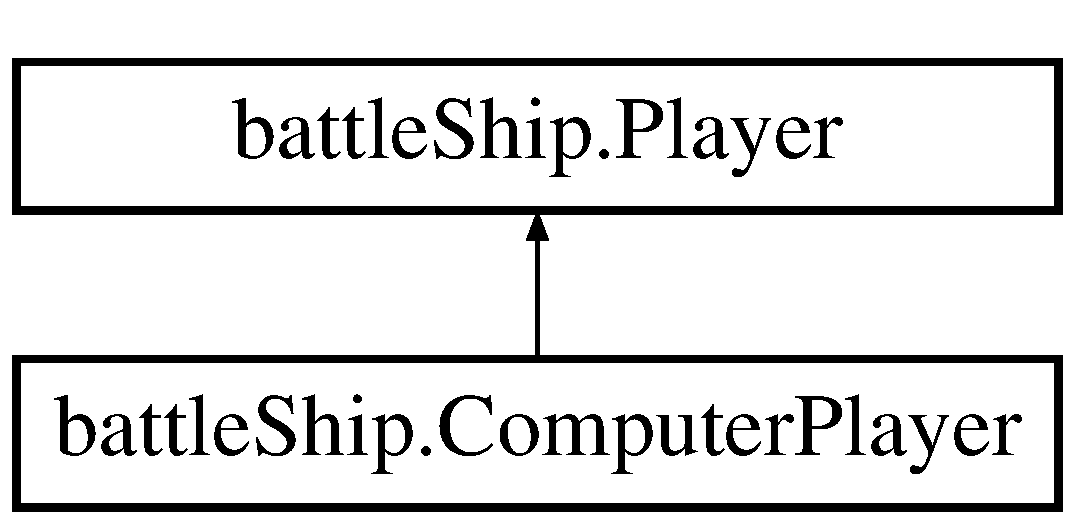
\includegraphics[height=2.000000cm]{classbattleShip_1_1ComputerPlayer}
\end{center}
\end{figure}
\subsection*{Public Member Functions}
\begin{DoxyCompactItemize}
\item 
\hyperlink{classbattleShip_1_1ComputerPlayer_a9158aa4d5add20abead9202ce3ef0ff2}{Computer\-Player} (int board\-Rows, int board\-Columns, int difficulty)
\begin{DoxyCompactList}\small\item\em Create a new \hyperlink{classbattleShip_1_1ComputerPlayer}{Computer\-Player} object. \end{DoxyCompactList}\item 
\hypertarget{classbattleShip_1_1ComputerPlayer_a23903e61dcd8593a21b24770e089dedf}{void {\bfseries prompt\-For\-Name} (int player)}\label{classbattleShip_1_1ComputerPlayer_a23903e61dcd8593a21b24770e089dedf}

\item 
\hypertarget{classbattleShip_1_1ComputerPlayer_a9d14fb18c9e81498a5c77b215d169642}{void {\bfseries setup\-Board} ()}\label{classbattleShip_1_1ComputerPlayer_a9d14fb18c9e81498a5c77b215d169642}

\end{DoxyCompactItemize}
\subsection*{Static Public Attributes}
\begin{DoxyCompactItemize}
\item 
\hypertarget{classbattleShip_1_1ComputerPlayer_a6c571d130881759c58dd164884e1d9f8}{static final int {\bfseries E\-A\-S\-Y} = 0}\label{classbattleShip_1_1ComputerPlayer_a6c571d130881759c58dd164884e1d9f8}

\item 
\hypertarget{classbattleShip_1_1ComputerPlayer_a91fb779591551636b1aa73e9dda09d99}{static final int {\bfseries M\-E\-D\-I\-U\-M} = 1}\label{classbattleShip_1_1ComputerPlayer_a91fb779591551636b1aa73e9dda09d99}

\item 
\hypertarget{classbattleShip_1_1ComputerPlayer_aa5904907d20a510c6fcfd7a008be18bf}{static final int {\bfseries H\-A\-R\-D} = 2}\label{classbattleShip_1_1ComputerPlayer_aa5904907d20a510c6fcfd7a008be18bf}

\end{DoxyCompactItemize}
\subsection*{Additional Inherited Members}


\subsection{Detailed Description}
This will implement an artificial player that can play Battleship. 

\begin{DoxyAuthor}{Author}
john 
\end{DoxyAuthor}


\subsection{Constructor \& Destructor Documentation}
\hypertarget{classbattleShip_1_1ComputerPlayer_a9158aa4d5add20abead9202ce3ef0ff2}{\index{battle\-Ship\-::\-Computer\-Player@{battle\-Ship\-::\-Computer\-Player}!Computer\-Player@{Computer\-Player}}
\index{Computer\-Player@{Computer\-Player}!battleShip::ComputerPlayer@{battle\-Ship\-::\-Computer\-Player}}
\subsubsection[{Computer\-Player}]{\setlength{\rightskip}{0pt plus 5cm}battle\-Ship.\-Computer\-Player.\-Computer\-Player (
\begin{DoxyParamCaption}
\item[{int}]{board\-Rows, }
\item[{int}]{board\-Columns, }
\item[{int}]{difficulty}
\end{DoxyParamCaption}
)}}\label{classbattleShip_1_1ComputerPlayer_a9158aa4d5add20abead9202ce3ef0ff2}


Create a new \hyperlink{classbattleShip_1_1ComputerPlayer}{Computer\-Player} object. 


\begin{DoxyParams}{Parameters}
{\em board\-Rows} & \\
\hline
{\em board\-Columns} & \\
\hline
{\em difficulty} & What difficulty should we play at? \\
\hline
\end{DoxyParams}
\begin{DoxySeeAlso}{See Also}
E\-A\-S\-Y 

M\-E\-D\-I\-U\-M 

H\-A\-R\-D 
\end{DoxySeeAlso}


The documentation for this class was generated from the following file\-:\begin{DoxyCompactItemize}
\item 
/home/john/\-Workspaces/\-Java/\-Battle-\/\-Ship/src/battle\-Ship/Computer\-Player.\-java\end{DoxyCompactItemize}

\hypertarget{classbattleShip_1_1HumanPlayer}{\section{battle\-Ship.\-Human\-Player Class Reference}
\label{classbattleShip_1_1HumanPlayer}\index{battle\-Ship.\-Human\-Player@{battle\-Ship.\-Human\-Player}}
}


This class represents a \hyperlink{classbattleShip_1_1HumanPlayer}{Human\-Player} that can play from a \hyperlink{classbattleShip_1_1Window}{Window}.  


Inheritance diagram for battle\-Ship.\-Human\-Player\-:\begin{figure}[H]
\begin{center}
\leavevmode
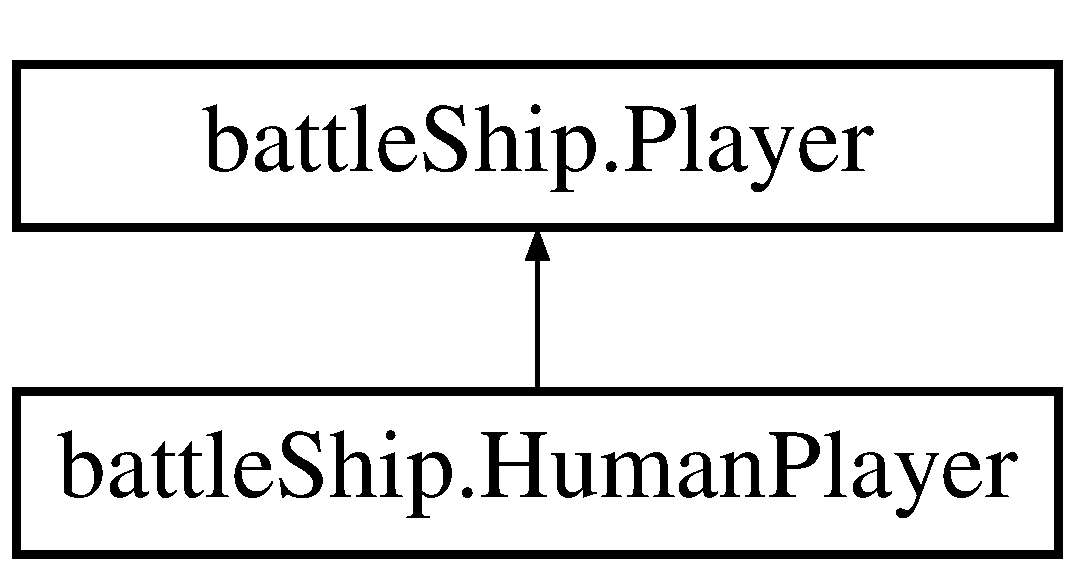
\includegraphics[height=2.000000cm]{classbattleShip_1_1HumanPlayer}
\end{center}
\end{figure}
\subsection*{Public Member Functions}
\begin{DoxyCompactItemize}
\item 
\hyperlink{classbattleShip_1_1HumanPlayer_a0e7b1784197eb8c8c80213d0b6e87660}{Human\-Player} (\hyperlink{classbattleShip_1_1Window}{Window} window, int board\-Rows, int board\-Columns)
\begin{DoxyCompactList}\small\item\em Create a human object with the given window for input, board rows and board columns. \end{DoxyCompactList}\item 
\hypertarget{classbattleShip_1_1HumanPlayer_a64c17bd80baa5f1b2bcb36b34d0746eb}{void \hyperlink{classbattleShip_1_1HumanPlayer_a64c17bd80baa5f1b2bcb36b34d0746eb}{prompt\-For\-Name} (int player)}\label{classbattleShip_1_1HumanPlayer_a64c17bd80baa5f1b2bcb36b34d0746eb}

\begin{DoxyCompactList}\small\item\em This will use the \hyperlink{classbattleShip_1_1Window}{Window} to get the player's name. \end{DoxyCompactList}\item 
\hypertarget{classbattleShip_1_1HumanPlayer_ac054fa48213ba59b14c105d686491df9}{void \hyperlink{classbattleShip_1_1HumanPlayer_ac054fa48213ba59b14c105d686491df9}{setup\-Board} ()}\label{classbattleShip_1_1HumanPlayer_ac054fa48213ba59b14c105d686491df9}

\begin{DoxyCompactList}\small\item\em Ask the player for their ship board configuration. \end{DoxyCompactList}\end{DoxyCompactItemize}
\subsection*{Additional Inherited Members}


\subsection{Detailed Description}
This class represents a \hyperlink{classbattleShip_1_1HumanPlayer}{Human\-Player} that can play from a \hyperlink{classbattleShip_1_1Window}{Window}. 

\begin{DoxyAuthor}{Author}
John Detter\href{mailto:john@detter.com}{\tt john@detter.\-com} 
\end{DoxyAuthor}


\subsection{Constructor \& Destructor Documentation}
\hypertarget{classbattleShip_1_1HumanPlayer_a0e7b1784197eb8c8c80213d0b6e87660}{\index{battle\-Ship\-::\-Human\-Player@{battle\-Ship\-::\-Human\-Player}!Human\-Player@{Human\-Player}}
\index{Human\-Player@{Human\-Player}!battleShip::HumanPlayer@{battle\-Ship\-::\-Human\-Player}}
\subsubsection[{Human\-Player}]{\setlength{\rightskip}{0pt plus 5cm}battle\-Ship.\-Human\-Player.\-Human\-Player (
\begin{DoxyParamCaption}
\item[{{\bf Window}}]{window, }
\item[{int}]{board\-Rows, }
\item[{int}]{board\-Columns}
\end{DoxyParamCaption}
)}}\label{classbattleShip_1_1HumanPlayer_a0e7b1784197eb8c8c80213d0b6e87660}


Create a human object with the given window for input, board rows and board columns. 


\begin{DoxyParams}{Parameters}
{\em window} & The window to get input from. \\
\hline
{\em board\-Rows} & How many board rows are there? \\
\hline
{\em board\-Columns} & How many board columns are there? \\
\hline
\end{DoxyParams}


The documentation for this class was generated from the following file\-:\begin{DoxyCompactItemize}
\item 
/home/john/\-Workspaces/\-Java/\-Battle-\/\-Ship/src/battle\-Ship/Human\-Player.\-java\end{DoxyCompactItemize}

\hypertarget{classbattleShip_1_1Player}{\section{battle\-Ship.\-Player Class Reference}
\label{classbattleShip_1_1Player}\index{battle\-Ship.\-Player@{battle\-Ship.\-Player}}
}


This base \hyperlink{classbattleShip_1_1Player}{Player} class is used as a template for it's children.  


Inheritance diagram for battle\-Ship.\-Player\-:\begin{figure}[H]
\begin{center}
\leavevmode
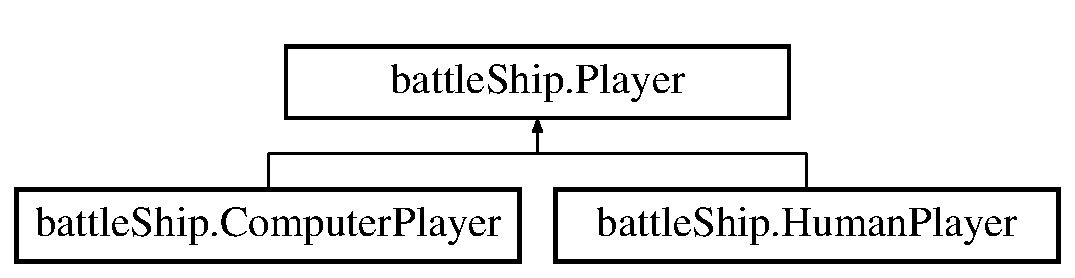
\includegraphics[height=2.000000cm]{classbattleShip_1_1Player}
\end{center}
\end{figure}
\subsection*{Public Member Functions}
\begin{DoxyCompactItemize}
\item 
\hyperlink{classbattleShip_1_1Player_a84d74412700d272b08418669be84f917}{Player} (int board\-Rows, int board\-Columns)
\begin{DoxyCompactList}\small\item\em Creates a new \hyperlink{classbattleShip_1_1Player}{Player} object and initializes guess\-Board, piece\-Board and name. \end{DoxyCompactList}\item 
void \hyperlink{classbattleShip_1_1Player_a777f39da73ac37362d259ba840e88fb2}{ready\-Player} (int player)
\begin{DoxyCompactList}\small\item\em Get the user ready for the game. \end{DoxyCompactList}\item 
abstract void \hyperlink{classbattleShip_1_1Player_a7d2073f6e08c56c500b1abac95345105}{prompt\-For\-Name} (int player)
\begin{DoxyCompactList}\small\item\em Prompt the user for the name they want to use. \end{DoxyCompactList}\item 
\hypertarget{classbattleShip_1_1Player_acb9e756832ce9afef891658d83c48713}{abstract void \hyperlink{classbattleShip_1_1Player_acb9e756832ce9afef891658d83c48713}{setup\-Board} ()}\label{classbattleShip_1_1Player_acb9e756832ce9afef891658d83c48713}

\begin{DoxyCompactList}\small\item\em Allow the player to place their pieces on the game board. \end{DoxyCompactList}\item 
\hypertarget{classbattleShip_1_1Player_a716a672218a3e61e143860c9e18947de}{boolean {\bfseries is\-Ready} ()}\label{classbattleShip_1_1Player_a716a672218a3e61e143860c9e18947de}

\item 
\hypertarget{classbattleShip_1_1Player_a85f80769be58bde359baf98eff289efe}{void {\bfseries set\-Name} (String \hyperlink{classbattleShip_1_1Player_a0be29098278ff1ccb8ebac1fc08546c2}{name})}\label{classbattleShip_1_1Player_a85f80769be58bde359baf98eff289efe}

\item 
\hypertarget{classbattleShip_1_1Player_a36a5c5c7485d2c05d36dccb19165fb84}{String {\bfseries get\-Name} ()}\label{classbattleShip_1_1Player_a36a5c5c7485d2c05d36dccb19165fb84}

\end{DoxyCompactItemize}
\subsection*{Protected Attributes}
\begin{DoxyCompactItemize}
\item 
\hyperlink{classbattleShip_1_1Board}{Board} \hyperlink{classbattleShip_1_1Player_ad3cfcbcfee296ba644ea8f385d878799}{guess\-Board}
\begin{DoxyCompactList}\small\item\em This board is used to show the guesses for the player. \end{DoxyCompactList}\item 
\hyperlink{classbattleShip_1_1Board}{Board} \hyperlink{classbattleShip_1_1Player_a57e76a8f3bb9739c402cad1f2eb1205a}{ship\-Board}
\begin{DoxyCompactList}\small\item\em This board is used to show the placement of the user's ships. \end{DoxyCompactList}\item 
String \hyperlink{classbattleShip_1_1Player_a0be29098278ff1ccb8ebac1fc08546c2}{name}
\begin{DoxyCompactList}\small\item\em The name of the player. \end{DoxyCompactList}\item 
boolean \hyperlink{classbattleShip_1_1Player_aeeb80baff53736294a7e406b8d19e1ac}{ready}
\begin{DoxyCompactList}\small\item\em Whether or not the player is ready to play. \end{DoxyCompactList}\end{DoxyCompactItemize}


\subsection{Detailed Description}
This base \hyperlink{classbattleShip_1_1Player}{Player} class is used as a template for it's children. 

All children need to implement \begin{DoxyAuthor}{Author}
john 
\end{DoxyAuthor}


\subsection{Constructor \& Destructor Documentation}
\hypertarget{classbattleShip_1_1Player_a84d74412700d272b08418669be84f917}{\index{battle\-Ship\-::\-Player@{battle\-Ship\-::\-Player}!Player@{Player}}
\index{Player@{Player}!battleShip::Player@{battle\-Ship\-::\-Player}}
\subsubsection[{Player}]{\setlength{\rightskip}{0pt plus 5cm}battle\-Ship.\-Player.\-Player (
\begin{DoxyParamCaption}
\item[{int}]{board\-Rows, }
\item[{int}]{board\-Columns}
\end{DoxyParamCaption}
)}}\label{classbattleShip_1_1Player_a84d74412700d272b08418669be84f917}


Creates a new \hyperlink{classbattleShip_1_1Player}{Player} object and initializes guess\-Board, piece\-Board and name. 


\begin{DoxyParams}{Parameters}
{\em board\-Rows} & How many rows are on the board? \\
\hline
{\em board\-Columns} & How many columns are on the board? \\
\hline
\end{DoxyParams}


\subsection{Member Function Documentation}
\hypertarget{classbattleShip_1_1Player_a7d2073f6e08c56c500b1abac95345105}{\index{battle\-Ship\-::\-Player@{battle\-Ship\-::\-Player}!prompt\-For\-Name@{prompt\-For\-Name}}
\index{prompt\-For\-Name@{prompt\-For\-Name}!battleShip::Player@{battle\-Ship\-::\-Player}}
\subsubsection[{prompt\-For\-Name}]{\setlength{\rightskip}{0pt plus 5cm}abstract void battle\-Ship.\-Player.\-prompt\-For\-Name (
\begin{DoxyParamCaption}
\item[{int}]{player}
\end{DoxyParamCaption}
)\hspace{0.3cm}{\ttfamily [abstract]}}}\label{classbattleShip_1_1Player_a7d2073f6e08c56c500b1abac95345105}


Prompt the user for the name they want to use. 


\begin{DoxyParams}{Parameters}
{\em player} & \\
\hline
\end{DoxyParams}
\hypertarget{classbattleShip_1_1Player_a777f39da73ac37362d259ba840e88fb2}{\index{battle\-Ship\-::\-Player@{battle\-Ship\-::\-Player}!ready\-Player@{ready\-Player}}
\index{ready\-Player@{ready\-Player}!battleShip::Player@{battle\-Ship\-::\-Player}}
\subsubsection[{ready\-Player}]{\setlength{\rightskip}{0pt plus 5cm}void battle\-Ship.\-Player.\-ready\-Player (
\begin{DoxyParamCaption}
\item[{int}]{player}
\end{DoxyParamCaption}
)}}\label{classbattleShip_1_1Player_a777f39da73ac37362d259ba840e88fb2}


Get the user ready for the game. 

This includes calling prompt\-For\-Name and setup\-Board. The completion of this method call does N\-O\-T require the player to be ready, it signifies that the player has started to get ready.


\begin{DoxyParams}{Parameters}
{\em player} & The player number. \\
\hline
\end{DoxyParams}
\begin{DoxySeeAlso}{See Also}
is\-Ready 
\end{DoxySeeAlso}


\subsection{Member Data Documentation}
\hypertarget{classbattleShip_1_1Player_ad3cfcbcfee296ba644ea8f385d878799}{\index{battle\-Ship\-::\-Player@{battle\-Ship\-::\-Player}!guess\-Board@{guess\-Board}}
\index{guess\-Board@{guess\-Board}!battleShip::Player@{battle\-Ship\-::\-Player}}
\subsubsection[{guess\-Board}]{\setlength{\rightskip}{0pt plus 5cm}{\bf Board} battle\-Ship.\-Player.\-guess\-Board\hspace{0.3cm}{\ttfamily [protected]}}}\label{classbattleShip_1_1Player_ad3cfcbcfee296ba644ea8f385d878799}


This board is used to show the guesses for the player. 

\hypertarget{classbattleShip_1_1Player_a0be29098278ff1ccb8ebac1fc08546c2}{\index{battle\-Ship\-::\-Player@{battle\-Ship\-::\-Player}!name@{name}}
\index{name@{name}!battleShip::Player@{battle\-Ship\-::\-Player}}
\subsubsection[{name}]{\setlength{\rightskip}{0pt plus 5cm}String battle\-Ship.\-Player.\-name\hspace{0.3cm}{\ttfamily [protected]}}}\label{classbattleShip_1_1Player_a0be29098278ff1ccb8ebac1fc08546c2}


The name of the player. 

\hypertarget{classbattleShip_1_1Player_aeeb80baff53736294a7e406b8d19e1ac}{\index{battle\-Ship\-::\-Player@{battle\-Ship\-::\-Player}!ready@{ready}}
\index{ready@{ready}!battleShip::Player@{battle\-Ship\-::\-Player}}
\subsubsection[{ready}]{\setlength{\rightskip}{0pt plus 5cm}boolean battle\-Ship.\-Player.\-ready\hspace{0.3cm}{\ttfamily [protected]}}}\label{classbattleShip_1_1Player_aeeb80baff53736294a7e406b8d19e1ac}


Whether or not the player is ready to play. 

\hypertarget{classbattleShip_1_1Player_a57e76a8f3bb9739c402cad1f2eb1205a}{\index{battle\-Ship\-::\-Player@{battle\-Ship\-::\-Player}!ship\-Board@{ship\-Board}}
\index{ship\-Board@{ship\-Board}!battleShip::Player@{battle\-Ship\-::\-Player}}
\subsubsection[{ship\-Board}]{\setlength{\rightskip}{0pt plus 5cm}{\bf Board} battle\-Ship.\-Player.\-ship\-Board\hspace{0.3cm}{\ttfamily [protected]}}}\label{classbattleShip_1_1Player_a57e76a8f3bb9739c402cad1f2eb1205a}


This board is used to show the placement of the user's ships. 



The documentation for this class was generated from the following file\-:\begin{DoxyCompactItemize}
\item 
/home/john/\-Workspaces/\-Java/\-Battle-\/\-Ship/src/battle\-Ship/Player.\-java\end{DoxyCompactItemize}

\hypertarget{classbattleShip_1_1Window}{\section{battle\-Ship.\-Window Class Reference}
\label{classbattleShip_1_1Window}\index{battle\-Ship.\-Window@{battle\-Ship.\-Window}}
}
Inheritance diagram for battle\-Ship.\-Window\-:\begin{figure}[H]
\begin{center}
\leavevmode
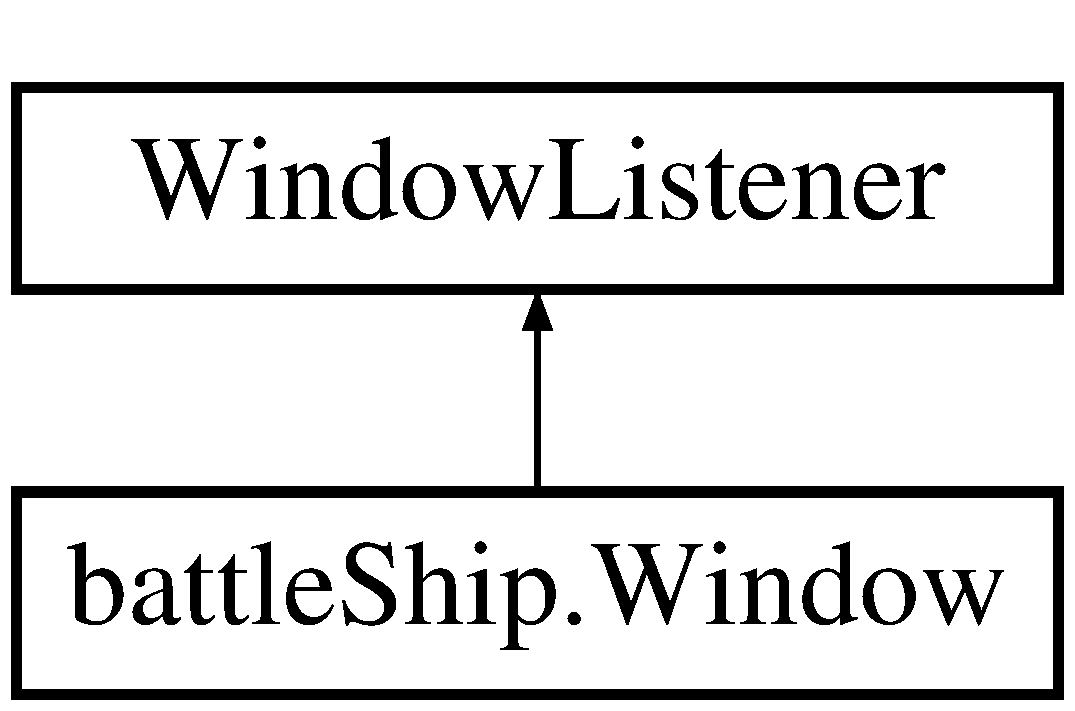
\includegraphics[height=2.000000cm]{classbattleShip_1_1Window}
\end{center}
\end{figure}
\subsection*{Public Member Functions}
\begin{DoxyCompactItemize}
\item 
\hypertarget{classbattleShip_1_1Window_a726b41baa3e2daf1eef7586eec390612}{{\bfseries Window} (int rows, int columns)}\label{classbattleShip_1_1Window_a726b41baa3e2daf1eef7586eec390612}

\item 
\hypertarget{classbattleShip_1_1Window_ac65bc743a1078760a9330078445ac6f7}{{\bfseries Window} (String title, int rows, int columns, boolean exit\-On\-Close)}\label{classbattleShip_1_1Window_ac65bc743a1078760a9330078445ac6f7}

\item 
\hypertarget{classbattleShip_1_1Window_a214a8387f89e8bd3f678c605416d4b3f}{void {\bfseries window\-Activated} (Window\-Event e)}\label{classbattleShip_1_1Window_a214a8387f89e8bd3f678c605416d4b3f}

\item 
\hypertarget{classbattleShip_1_1Window_afe7561ad4e2cf55deeeb41033ab4d998}{void {\bfseries window\-Closed} (Window\-Event e)}\label{classbattleShip_1_1Window_afe7561ad4e2cf55deeeb41033ab4d998}

\item 
\hypertarget{classbattleShip_1_1Window_a111c1da295b878bdb046c6aadc010e84}{void {\bfseries window\-Deactivated} (Window\-Event e)}\label{classbattleShip_1_1Window_a111c1da295b878bdb046c6aadc010e84}

\item 
\hypertarget{classbattleShip_1_1Window_a6f114e4e446e31e6a772172e3c63ecdd}{void {\bfseries window\-Deiconified} (Window\-Event e)}\label{classbattleShip_1_1Window_a6f114e4e446e31e6a772172e3c63ecdd}

\item 
\hypertarget{classbattleShip_1_1Window_a20e8082132fcfaa5027a83284eb0abac}{void {\bfseries window\-Iconified} (Window\-Event e)}\label{classbattleShip_1_1Window_a20e8082132fcfaa5027a83284eb0abac}

\item 
\hypertarget{classbattleShip_1_1Window_a40bf9fda41c424ca5bf52d371da79a5f}{void {\bfseries window\-Opened} (Window\-Event e)}\label{classbattleShip_1_1Window_a40bf9fda41c424ca5bf52d371da79a5f}

\item 
\hypertarget{classbattleShip_1_1Window_ae2826f39804482199ccb2b3f9ee8ed21}{void {\bfseries window\-Closing} (Window\-Event e)}\label{classbattleShip_1_1Window_ae2826f39804482199ccb2b3f9ee8ed21}

\item 
\hypertarget{classbattleShip_1_1Window_ac820eeb047f63e50b38ed572e7bea2a3}{void {\bfseries print} (final String s)}\label{classbattleShip_1_1Window_ac820eeb047f63e50b38ed572e7bea2a3}

\item 
\hypertarget{classbattleShip_1_1Window_a63d6fe9640b210238e4d1b9fd04effc7}{void {\bfseries println} ()}\label{classbattleShip_1_1Window_a63d6fe9640b210238e4d1b9fd04effc7}

\item 
\hypertarget{classbattleShip_1_1Window_abdaeade215ae95f8684ec6450a672c6d}{void {\bfseries println} (final String s)}\label{classbattleShip_1_1Window_abdaeade215ae95f8684ec6450a672c6d}

\item 
\hypertarget{classbattleShip_1_1Window_abf2ff42e8976cd34ce6ca1f8e4d00268}{String {\bfseries next\-Line} ()}\label{classbattleShip_1_1Window_abf2ff42e8976cd34ce6ca1f8e4d00268}

\item 
\hypertarget{classbattleShip_1_1Window_ae954372a5fc388c81b2b428bc5c01f7f}{int {\bfseries next\-Int} ()}\label{classbattleShip_1_1Window_ae954372a5fc388c81b2b428bc5c01f7f}

\item 
\hypertarget{classbattleShip_1_1Window_a683f5733202653718286209f6e7ab5ca}{long {\bfseries next\-Long} ()}\label{classbattleShip_1_1Window_a683f5733202653718286209f6e7ab5ca}

\item 
\hypertarget{classbattleShip_1_1Window_af3d2929699fbf63c1ea7a05a1e0fd2ee}{float {\bfseries next\-Float} ()}\label{classbattleShip_1_1Window_af3d2929699fbf63c1ea7a05a1e0fd2ee}

\item 
\hypertarget{classbattleShip_1_1Window_a2a798787bb6e52698ddcc1479b07c751}{double {\bfseries next\-Double} ()}\label{classbattleShip_1_1Window_a2a798787bb6e52698ddcc1479b07c751}

\item 
\hypertarget{classbattleShip_1_1Window_a444c42bf30aefa08006bb2c80b2dedbf}{short {\bfseries next\-Short} ()}\label{classbattleShip_1_1Window_a444c42bf30aefa08006bb2c80b2dedbf}

\item 
\hypertarget{classbattleShip_1_1Window_a16f9f3d7c222bb91dd1a9c6d7f131941}{void {\bfseries clear} ()}\label{classbattleShip_1_1Window_a16f9f3d7c222bb91dd1a9c6d7f131941}

\item 
\hypertarget{classbattleShip_1_1Window_a233909005709f7c5063b352ccdd41af0}{boolean {\bfseries prompt} ()}\label{classbattleShip_1_1Window_a233909005709f7c5063b352ccdd41af0}

\item 
\hypertarget{classbattleShip_1_1Window_aee61a29762bf0fa617894920f836326b}{void {\bfseries reset\-Latch} ()}\label{classbattleShip_1_1Window_aee61a29762bf0fa617894920f836326b}

\end{DoxyCompactItemize}


The documentation for this class was generated from the following file\-:\begin{DoxyCompactItemize}
\item 
/home/john/\-Workspaces/\-Java/\-Battle-\/\-Ship/src/battle\-Ship/Window.\-java\end{DoxyCompactItemize}

%--- End generated contents ---

% Index
\newpage
\phantomsection
\addcontentsline{toc}{chapter}{Index}
\printindex

\end{document}
